\chapter{Applications, Summary and Conclusions}\label{chap:conclusions}

This chapter aims to present a concrete application of the singing voice pronunciation assessment and results presented in the previous chapters. The application section is followed by a summary of the work presented in the thesis, along with some key results and conclusions. The last section opens up some open problems and directions for future work. 

\section{Applications}

There are quite a few applications for the research work presented in the thesis. Some of these applications have been identified in \chapref{chap:intro}. This section aims to present concrete examples of such applications and further propose other applications that might be built from the thesis work. This section also describes in detail one application that has resulted from the work in MusicCritic\footnote{\url{https://musiccritic.upf.edu/}} project. Possible future applications are also discussed briefly.

The primary objective and application of the methodologies related to automatic singing voice assessment -- syllable and phoneme segmentation, mispronunciation detection and pronunciation and overall similarity measures, is to use them for online or on-site singing voice training. Additionally, there are many ways to use the methodologies developed in this thesis for various applications.

Jingju singing exercises can be organized into melodic lines in an online jingju singing teaching course. The teacher's singing recordings are provided in the exercise as the demonstrative singing example. The students who take this exercise are required to imitate the teacher's singing. To automatically assess the imitative singing of the students, the assessment tools can segment the student's recording into syllable and phoneme units, detect the mispronunciation for special pronunciation and jiantuanzi syllables, and measure the pronunciation and overall quality similarities between teacher's and student's singing phonemes. The assessment results can serve as initial guidance for the students to improve their singing skills in the absence of a singing instructor.

The methods developed in this thesis also have the potential to be applied in the on-site jingju singing training scenario. As it has been mentioned in \secref{sec:probdef:role_pronunciation}, jingju singing is taught between teacher and student by using the oral teaching and face-to-face methods. The students need to understand the teacher's verbal or singing feedbacks firstly, assimilate them, then do a lot of singing practice to improve their singing skills. However, the teacher's verbal feedback is usually mixed with many personal comments (check the teacher's feedbacks in correction occurrence in \secref{sec:probdef:correction_occurance}), and thus cannot describe the student's singing problems in an objective and precise way. The syllable and phoneme segmentation method developed in our thesis can automatically segment and label the teacher's singing melodic line into syllable or phoneme units. With the help of some singing voice or speech visualization technologies, such as pitch, loudness tracking, formant frequency tracking, the students could better assimilate the teacher's verbal feedback by benefiting from the visual cues of their singing voice segmented into syllable and phoneme units.

Automatic singing voice assessment technologies find their application in helping navigate through jingju singing voice recordings and in content-based music retrieval. Applications such search by pronunciation traits can be conceived, such as query by mispronunciation rate, query by pronunciation similarity. Additionally, the automatic syllable and phoneme segmentation method applied on the jingju singing recordings allows a clear visualization of the syllable/phoneme boundaries and labels, which could be applied to a semantic exploration of the singing corpus.

Musicologists working with jingju pronunciation would benefit from the corpora and tools developed in this thesis. The jingju a cappella singing voice datasets are representative and well-curated with useful metadata, annotations, and can be used to derive musicological findings. Automatic syllable and phoneme segmentation tool can lead to a precise segmentation of the singing syllable/phoneme units and hence to analyze large corpora of recordings, which would be otherwise time-consuming if done manually. The mispronunciation detection tool is useful to annotate automatically the pronunciation correctness of the singing recordings at syllable level, which could be interesting to the musicologists who study the pronunciation trait of the jingju singing.

To conclude, one specific application built with MusicCritic project is described below -- sofège assessment. This application is the collaborative effort of the MusicCritic team. A brief introduction to the application is provided, and then we put stress on how the pronunciation assessment methods developed in this thesis applied and integrated into this application.

\subsection{MusicCritic solfège assessment}

MusicCritic is a music performance technology with which to evaluate musical exercises sung or played by students, giving meaningful feedback. It is a service that uses the Basic LTI standard\footnote{\url{http://www.imsglobal.org/activity/learning-tools-interoperability}} and can be easily integrated into online applications or education platforms, such as Coursera\footnote{\url{https://www.coursera.org/}} and Kadenze\footnote{\url{https://www.kadenze.com/}}. It contains four sub-technologies -- solfège, melodic imitation, chord playing and improvisation assessment, developed collaboratively by the researchers and developers in MTG. The solfège assessment tool stems from the automatic singing voice segmentation and assessment methods conceived in this thesis. 

MusicCritic solfège assessment tool can receive the student's solfège singing recording, then return the pitch, rhythm and pronunciation feedback visually and automatically. It also generates the pitch and pronunciation assessment scores for the student's recording. With the help of the MusicCritic LTI standard integration, the solfège assessment tool can be easily integrated into online applications or education platforms that support this standard.

The research results from this thesis on singing voice assessment are partly integrated into MusicCritic solfège assessment tool. A Kaldi-based syllable recognition system extended from the mispronunciation detection baseline presented in \secref{sec:ch6:forced_alignment} is used to recognize the solfège syllable and detect its boundaries. The pitch, rhythm and pronunciation accuracy visualization is done based on the recognition results.

\begin{landscape}
\mbox{}\vfill
\begin{figure}[ht!]
    \centering
    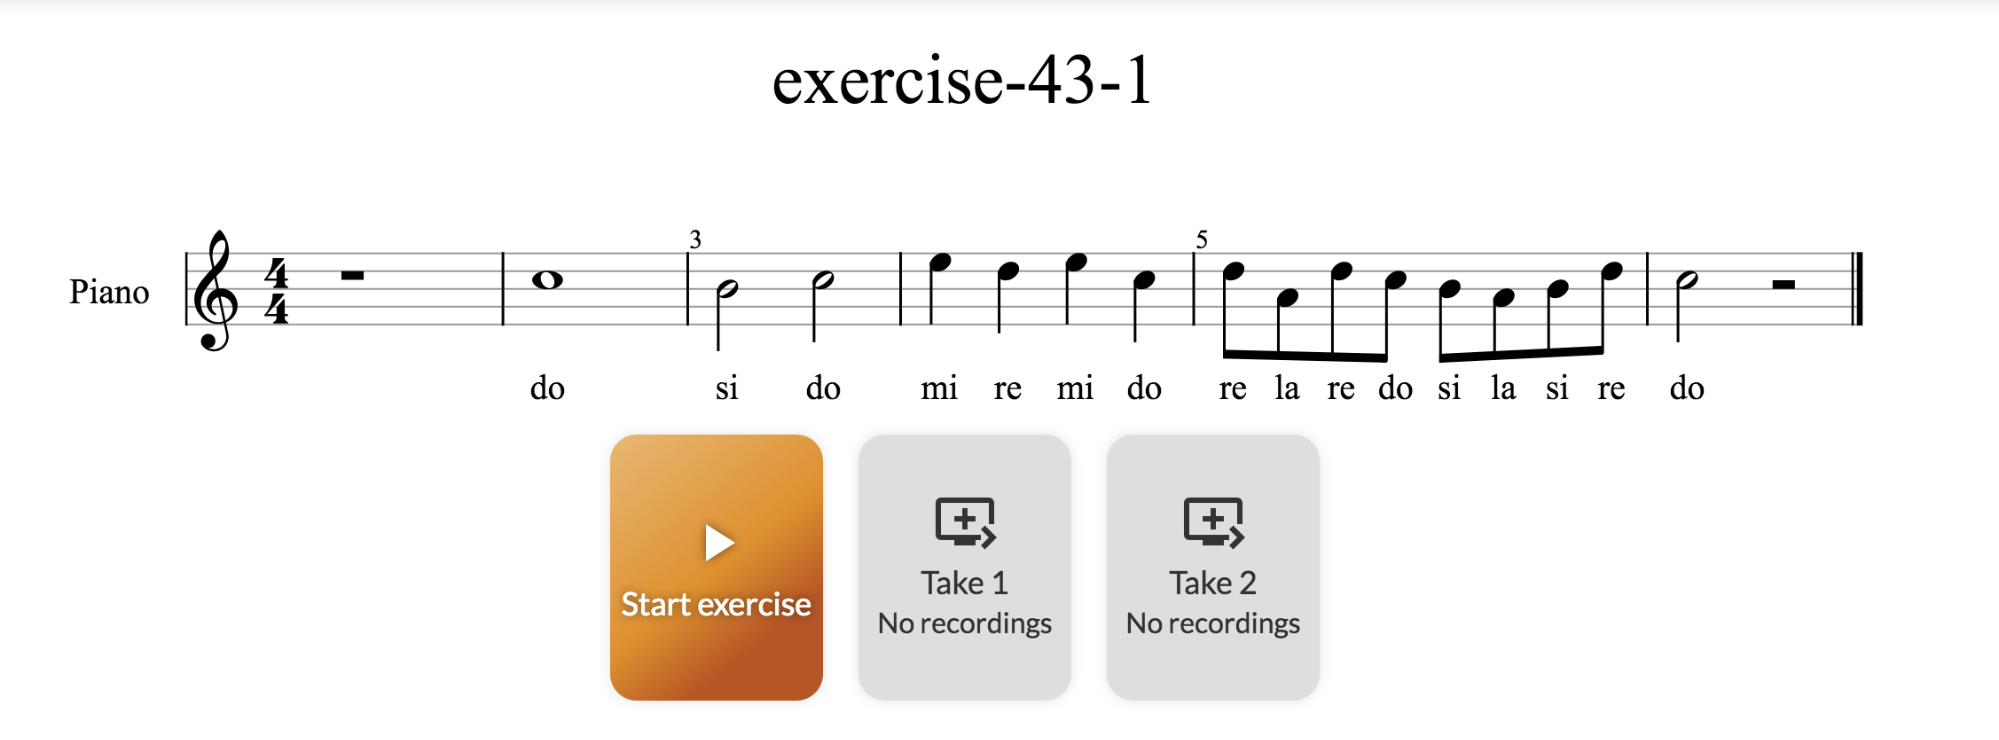
\includegraphics[width=1.8\textwidth]{figs/ch8/ch8_mc1.png}
    \caption{A screenshot of the recording page of the solège assessment tool. The student can listen the demonstrative singing by clicking ``Start exercise", then record their singing twice by clicking ``Take 1" and ``Take 2" buttons.}
    \label{fig:ch8:recording_interface}
\end{figure}
\vfill
\end{landscape}

\begin{landscape}
\mbox{}\vfill
\begin{figure}[ht!]
    % \centering
    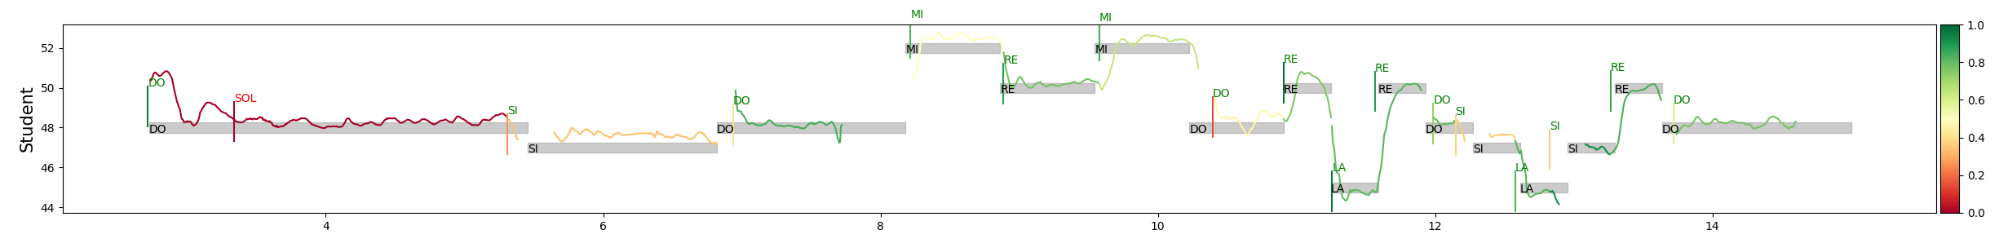
\includegraphics[width=1.8\textwidth]{figs/ch8/ch8_mc2.png}
    \caption{The visualzation of a student's recording. The rectangles in grey are the ground truth solfège notes of which the name is labeled at the beginning of each note. The curve indicates the pitch. The vertical lines before each detected notes indicate the note onset positions. The character on top of the vertical line indicates the detected note name. The singing quality is indicated by the color system -- green: good performance, red: bad performance.}
    \label{fig:ch8:eval_visual}
\end{figure}
\vfill
\end{landscape}

\figref{fig:ch8:recording_interface} shows a recording interface of the solfège assessment tool, where the student can listen to the demonstrative singing recording, then record and submit their singing voice to the assessment tool. \figref{fig:ch8:eval_visual} shows the assessment result visualization automatically generated by the tool on which the singing quality of three aspects -- pitch, note onset and pronunciation, are visualized by the color system.

\section{Contributions}

A summary of the specific contributions from the work presented in the thesis is listed below.

\subsection{Contributions to creating research corpora and datasets}

Building research corpora for MIR is one of the primary tasks of CompMusic project. Significant efforts have been put into building research corpora and datasets. The relevant datasets are listed below. The link to access all these datasets are provided in Appendix

\begin{itemize}[leftmargin=*]
\item Automatic syllable and phoneme segmentation (ASPS) dataset (\secref{sec:ch4:dataset_segmentation}): This dataset has two sub-datasets (ASPS\textsubscript{1} and ASPS\textsubscript{2}) which contain in total 197 jingju singing recordings. Each recording in ASPS\textsubscript{1} is annotated with syllable and phoneme boundaries and labels. While the recordings in ASPS\textsubscript{2} are annotated at syllable-level. The annotation is done by the author with the support of Rafeal Caro Repetto and Yile Yang.
\item Mispronunciation detection (MD) dataset (\secref{sec:ch4:dataset_mispronunciation}): Special pronunciation, jiantuanzi syllables and the mispronunciation labels for these two types of the syllable are annotated for 1007 jingju singing melodic lines in this dataset.
\item Pronunciation and overall quality similarity measures (POQSM) dataset (\secref{sec:ch4:poqsm_dataset}): This dataset contains 19911 jingju singing phoneme segments recorded by both professional and amateur singers. These segments are split deliberately to build pronunciation and overall quality similarity models.
\end{itemize}

\subsection{Technical and scientific contributions}

\begin{itemize}[leftmargin=*]
\item Identification of the critical role of pronunciation in jingju singing training (\secref{sec:probdef:role_pronunciation}).
\item Identification of challenges, opportunities and applications of automatic singing voice pronunciation assessment of jingju music (\secref{sec:ch3:challenges_opportunities}).
\item Identification of four problems which are the most relevant to automatic singing voice pronunciation assessment of jingju music, along with a review of the state-of-the-art methods (\secref{sec:ch3:research_problems}). 
\item Formulation the problems of automatic syllable and phoneme segmentation, mispronunciation detection, and pronunciation and overall quality similarity measures in jingju music (\secref{sec:ch3:formulation}).
\item An evaluation of the jingju a cappella singing corpus based on the methodology by Serra \cite{Serra2014} (\secref{sec:ch4:compmusic_corpora}).
\item A demonstration of the utility of corpus for musicological analysis -- melodic line, syllable and phoneme duration analysis (\secref{sec:ch4:dataset_analysis}).
\item Duration-informed syllable and phoneme segmentation for jingju singing. Developing approaches that combine the feature learning power of the deep learning models and the inference the syllable or phoneme onset positions by using the coarse duration information explicitly. New onset selection HMM model is proposed, which shows improvement in both syllable or phoneme onset detection and segmentation (\chapref{chap:segmentation}).
\item Demonstration of the validity of applying deep learning-based classification models in mispronunciation detection of jingju singing syllables (\chapref{chap:mispronunciation}). 
\item Phoneme embedding-based approaches for measuring pronunciation and overall quality similarities at phoneme-level (\secref{chap:similarity_pronunciation}).
\end{itemize}

\section{Summary and conclusions}

In this section, we present a summary, conclusions and the key results from the thesis, organized based on the chapters of the thesis. Broadly, the thesis aimed to build culture-specific data-driven MIR approaches using deep learning and probabilistic models for automatic pronunciation assessment in jingju music, focusing mainly on the tasks of syllable and phoneme segmentation, mispronunciation detection and pronunciation and overall quality similarity measures. Such approaches would lead to tools and technologies that can improve our experience of jingju singing training, within the context of jingju music culture. The applications lie in computer-aided jingju singing training, music navigation, content-based music retrieval and musicology, and as pre-processing steps for MIR tasks extracting semantic information such as singing syllable and phoneme.

This thesis focused on automatic singing voice pronunciation assessment tasks within the scope of CompMusic project, which is limited to developing data collections and computational models for singing voice pronunciation assessment in jingju music.

An introduction to singing in jingju art music was presented in \chapref{chap:bkgnd} with the concentration on jingju singing pronunciation concepts. The introduction provided a background to music concepts encountered in this thesis. A comparison of the pronunciation characteristics between jingju singing and Western opera singing showed the contrasting differences between two singing genres. A review of state of the art in automatic singing voice pronunciation assessment-related tasks provided a basis for understanding relevant methodologies in jingju singing.

\chapref{chap:probdef} identified the critical role of pronunciation in jingju singing training, and thus justified the pronunciation assessment as the main focus of this thesis. Additionally, this chapter identified some of the challenges and opportunities of jingju singing pronunciation assessment. Important and relevant research problems in the assessment of singing voice pronunciation of jingju music were identified and described, which will be useful to a researcher who is looking to solve relevant problems in this area of research.

Four core research problems -- building data corpus, syllable and phoneme segmentation, mispronunciation detection, and pronunciation and overall quality similarity measures, are formulated.

The problem of creating research corpora and datasets for data-driven MIR research, addressed in \chapref{chap:datasets} shows that significant efforts to build relevant datasets for automatic singing voice assessment research. The corpora and datasets are built and evaluated according to a set of corpus design criteria and methodologies. Furthermore, both corpus-level and dataset-level data analysis and visualization were conducted to draw some musicological inferences. To promote the idea of open data and reproducible research, the presented corpus, test datasets including audio recordings, metadata and annotations are openly available through Zenodo.org.

Automatic syllable and phoneme segmentation were one of the main problems addressed in this thesis. \chapref{chap:segmentation} presented a comprehensive methodology of syllable/phoneme onset detection and segmentation for jingju singing voice. The experiment on the baseline HSMM-based method showed an unideal performance on syllable/phoneme onset detection or segmentation tasks, indicating the need for a better method that can use the a priori coarse syllable/phoneme duration information. The duration-informed syllable/phoneme detection-based segmentation method that allows incorporating the coarse durations into the syllable and phoneme decoding process.

An evaluation of the duration-informed onset detection-based segmentation method clearly showed the improvement in both onset detection and segmentation tasks, compared with HSMM-based method. Additionally, the HMM onset selection model used in the proposed method allows a faster inference than the HSMM-based method. The segmentation performance depends on the goodness of the onset detection function. An exploration of various onset detection functions generated by different deep learning architectures showed that the onset detection function outputted from a basic convolutional architecture can achieve the state of the art segmentation accuracy, and is more efficient than other more complicated architectures. Lastly, the proposed segmentation model is capable of generalizing to other singing voice in languages different from Mandarin Chinese since its language-independency.

The mispronunciation detection problem for jingju singing was addressed in \chapref{chap:mispronunciation}. The task scope was constrained to the syllable-level special pronunciation and jiantuanzi mispronunciation detection because they are the primary source of the mispronounced syllables in jingju singing training. A forced-alignment baseline method and the proposed discriminative model-based method were experimented to tackle this problem.

The baseline method used a pronunciation dictionary with multiple pronunciations for each syllable entry. The mispronunciation detection worked as that the model decoding algorithm select the pronunciation which is matched best to the acoustics of the singing. The experiment on the baseline method showed a mediocre performance on special pronunciation syllable mispronunciation detection, and an unsatisfactory performance on jiantuanzi syllable mispronunciation detection.

The proposed method used firstly the syllable segmentation method presented in \chapref{chap:segmentation} to segment the singing recording into the syllable units, then used deep learning-based discriminative models to classify binarily the syllable units into mispronunciation or correct pronunciation class. Several deep learning techniques and two new architectures were experimented to augment the classification and generalization abilities. The results showed that the discriminative model-based method improved the mispronunciation detection accuracy on jiantuanzi syllables. The additional visualization of the attention vector showed that the attention mechanism worked well in making the classification decision based on certain essential regions of a syllable.

A framework for measuring pronunciation and overall quality similarities for jingju singing phoneme, along with an exploratory experiment was the subject matter of \chapref{chap:similarity_pronunciation}. Utilizing the phoneme embedding allows us to convert the variable-length syllable segments into fixed-length embedding vectors. The similarity measure can then be obtained by calculating the distance metric between two phoneme embeddings. 

An RNN-based classification model was proposed to generate the phoneme embedding. The model predicted the input phoneme segment into (1) different phonetic categories and (2) professional or amateur singing categories. The penultimate layer output was taken as the phoneme embedding as it was expected to embed the (1) phonetic and (2) overall quality information of the phoneme segment. Various deep learning techniques were experimented to improve the quality of the similarity measure and the generalization ability of the model. As an exploratory experiment, a siamese network which is designed originally for measuring the similarity between multiple inputs was tested. However, the performance was much worse than the classification model, and further experiments is needed to suggest improvements.

\section{Future directions}

There are several directions for future work based on the thesis. One of the goal of the thesis was to present relevant research problems in pronunciation assessment of jingju singing voice. Some of these problems presented in \secref{sec:ch3:research_problems} are a good start to extend the work presented in the thesis. Several tasks for jingju singing voice pronunciation assessment were proposed, while only a part of them was addressed in this thesis. The problems such as banshi (metrical structure) segmentation, melodic line segmentation, and automatic intonation or rhythm assessment have received little attention from the research community so far.

Automatic singing voice assessment of jingju music is a very board topic, and the assessment can be done in several musical dimensions, such as intonation, rhythm, loudness and pronunciation. The musical dimension which has been addressed extensively is pronunciation. The automatic assessment methods of the other musical dimensions related to jingju singing are worth to be explored in furture. Besides, the work in the thesis used mainly audio recordings along with syllable/phoneme duration and pronunciation annotations to develop computational models for the assessment. However, using additional information such as score, editorial metadata may lead to better automatic assessment models.

The curated a cappella jingju singing voice corpus and test data provide an opportunity to be used for a variety of research problems in future, such as jingju Query-by-singing, jingju singing transcription and jingju singing synthesis. The research corpus evolves. Improving the research corpus and building additional datasets for automatic jingju singing assessment are important tasks for the future. The use of the corpus and the datasets for musicological research was hinted in the thesis. However, a rigorous study of the suitability of the corpus and datasets for musicology, and comprehensive musicological research using the corpus is one direction to pursue in future.

Syllable and phoneme segmentation task was addressed in detail in the thesis. However, several open questions still need more exploration. The presented onset detection-based segmentation method can be extended by incorporating more side information other than duration, such as linguistic information. While the performance of the baseline lyrics-to-audio alignment method can be improved by including syllable/phoneme duration or onset information. The current onset detection-based segmentation method can deal with the situation that missing or extra syllables are sung in the recording. To develop a recognition-based method for the segmentation is a path to explore in future.

The mispronunciation detection task was addressed in the thesis with a preliminary result presented on a small dataset. The discriminative model-based detection method used deep learning architectures which require a large of training data to outperform the forced alignment-based method. To expand the amount of the training set by collecting more singing recordings, and reevaluate these two methods is a work to be done in future. 

The tasks of phoneme segmentation and pronunciation similarity measure were addressed as independent tasks in the thesis. An overall assessment of the similarity measurement pipeline requires to combine these two tasks. Additionally, the experiment results of using the siamese network in similarity measure are very preliminary. Extensive experiments to study this architecture including accelerating the model training, studying different data preparation methods need to be done in future.

Integration of these algorithms into practical applications requires additional effort. The evaluation of the validity of the integrated applications needs to be conducted in the real jingju singing training scenario. In the future, an integration of all the described singing voice pronunciation assessment approaches into one application is necessary and it helps to improve the algorithms through user feedback. 
